% AEGIS academic submission draft. Check factual claims, author details, and AI-use declaration before submitting.
% Source results trace to bundled archived AEGIS research reports (see Evidence/RESULTS_TRACEABILITY.md).
\documentclass[conference,a4paper]{IEEEtran}
\usepackage{graphicx}
\usepackage{booktabs}
\usepackage{amsmath}
\usepackage{array}
\usepackage{url}
\usepackage{balance}
\usepackage[T1]{fontenc}
\usepackage[utf8]{inputenc}
\usepackage{microtype}
\setlength{\emergencystretch}{2em}
\begin{document}
\title{AEGIS: Evidence-Grounded Predictive Research and Capacity-Constrained Decision Support for Supply-Chain Resilience}
\author{\IEEEauthorblockN{Arin Bakshi}
\IEEEauthorblockA{PGDM -- Big Data Analytics\\
Goa Institute of Management, Goa, India\\
Student ID: B2026119}}
\maketitle
\begin{abstract}
Disrupted fulfillment and uncertain supplier availability complicate supply-chain decisions. AEGIS is a local research prototype joining retrospective delivery-risk classification, synthetic supplier-allocation optimization, and an evidence-grounded managerial interface. In a public Brazilian e-commerce dataset, 38 supervised classifier configurations were benchmarked on 43,426 historically labeled training orders and 7,069 January 2018 selection orders. L2-regularized logistic regression achieved average precision (AP) of 0.145852 against a 0.057009 prevalence baseline, with ROC-AUC 0.690373. However, the same selected model's later historical checks yielded ROC-AUC 0.634753 (March) and 0.678720 (April--July), while calibration remained unreliable. Separately, an exact allocator solved a \emph{synthetic} 16-order supplier assignment with hard monthly capacities, reducing modeled cost from USD 1,928,061 to USD 1,698,024 under the stated fictional assumptions. A locally executed interface supports data upload, descriptive charts, source-checked explanations, and an optional on-device language model. The contribution is an auditable separation of observed data, research predictions, and hypothetical decisions; neither supplier savings nor prospective predictive reliability is established.
\end{abstract}
\begin{IEEEkeywords}
supply-chain resilience, decision intelligence, classification, prescriptive analytics, reproducibility, human-in-the-loop
\end{IEEEkeywords}

\section{Introduction}
Supply chains must make sourcing and fulfillment decisions despite delivery uncertainty, fixed capacities, and incomplete operational evidence. A dashboard alone describes what happened; a classifier ranks possible late deliveries; an optimizer can evaluate alternatives \emph{if} its assumptions and constraints are valid. Combining these layers is attractive, but confusing predicted risk with causal supplier performance can produce misleading recommendations. The distinction between predictive signals and operational prescriptions is fundamental to prescriptive analytics \cite{bertsimas2020}.

This study asks whether a single research system can (i) benchmark retrospective delivery-risk ranking, (ii) demonstrate auditable capacity-constrained allocation on declared scenarios, and (iii) explain findings to managers without presenting simulated benefits as realized outcomes. AEGIS's claimed originality is \emph{workflow integration and evidence separation}, not a new classifier or proof of a commercially deployable decision policy. Its design separates historical Olist records, fictional supplier planning inputs, and user-uploaded descriptive datasets. Procurement execution is disabled and human approval is required for any potential future use.

\section{Related Work}
Bertsimas and Kallus \cite{bertsimas2020} describe how observational data can inform decision prescriptions while emphasizing the relationship between data and decision quality. Predictive assessment itself requires care: Fawcett \cite{fawcett2006} explains ROC analysis, whereas Saito and Rehmsmeier \cite{saito2015} show why precision--recall analysis is particularly informative for imbalanced classifications. AEGIS therefore selects a historical classifier using AP, reports ROC-AUC as an additional discrimination measure, and examines calibration separately.

Operationalizing machine learning introduces data dependencies, validation drift, and other maintenance risks \cite{sculley2015}. Consequently, the prototype preserves immutable historical evidence and permits research-only scoring rather than automatically translating a model output into sourcing actions. The Olist public e-commerce dataset \cite{olist2018} supplies a reproducible historical setting, but it is not a source of authenticated supplier quotations, available capacities, or verified contractual service levels. The separate synthetic optimization experiment illustrates a decision framework, not an empirical causal evaluation.

\section{Methodology}
\subsection{Evidence Segmentation and Dataset}
AEGIS uses three distinct evidence lanes. First, historical Olist orders, customers, items, and sellers support a retrospective classification target: a comparable recorded delivery date later than the recorded estimated delivery date. The archived Olist order registry contains 99,441 records; an earlier frozen score audit retains 58,911 strictly comparable scored orders. These are not the same cohorts as the newer 2017--2018 classifier benchmark. Second, a fictional integrated planning dataset defines supplier prices, eligibility, lanes, capacities, and orders. Third, manager-uploaded CSV/XLSX data (or a selected authorized read-only SQLite table) support descriptive summaries and charts, \emph{not} unrestricted prediction or procurement.

\subsection{Historical Model Benchmark}
The expanded model study uses 43,426 mature, comparable orders from 2017 for development and 7,069 January 2018 orders for model selection. Thirty-eight fixed classifier configurations span regularized logistic regression, linear support-vector methods, tree ensembles, boosted trees, neural networks, naive Bayes, discriminant analysis, and other suitable classifiers. The selection rule prioritizes January AP and then ROC-AUC. The chosen L2 logistic model uses 65 candidate checkout features, including purchase-calendar signals, location, estimated-delivery horizon, item composition, quoted item price, and freight. Actual delivery date, reviews, and post-delivery status are excluded as input features. Nevertheless, original \emph{as-of} availability of several proposed checkout features was not independently witnessed, so feature validity remains provisional.

February 2018 is used to fit a sigmoid score calibration. March and April--July provide retrospective diagnostics; those periods had been viewed during iterative research and \emph{must not} be described as a new, untouched holdout. The historical classification study does not identify causal supplier effects. Since the target is relatively rare in January (403 delayed among 7,069 comparable records), the prevalence AP baseline of 0.057009 is an important comparator.

\subsection{Synthetic Decision Optimization}
A separate July 2025 synthetic case specifies 16 unsplittable component orders (13,900 units), one selected supplier per order, approved supplier--plant lanes, qualifications, minimum order quantities, and hard supplier--component monthly capacities. The research solver minimizes declared landed cost over eligible assignments:
\begin{equation}
\min_{x} \sum_{o\in\mathcal O}\sum_{s\in\mathcal S_o}c_{os}x_{os}
\end{equation}
subject to $\sum_{s\in\mathcal S_o}x_{os}=1$ for every order $o$, $\sum_o q_o x_{os}\leq C_s$ for each modeled supplier capacity, and $x_{os}\in\{0,1\}$. Ineligible pairs are excluded. The solution was cross-checked with an independent 0--1 reference on this bounded instance. Additional shared-shock sensitivity experiments cover 500 synthetic scenarios, 80 order--supplier pairs, and 40,000 paired exposure records. These shocks are assumed stress indices, not estimated delivery probabilities or observed disruptions.

\subsection{Application and Safeguards}
The local manager-facing application follows \emph{Data $\rightarrow$ Visualizations $\rightarrow$ Decision Copilot}. It provides descriptive data profiles, adaptive/custom charting and evidence-linked natural-language explanations; optional Ollama/Qwen supplies a local conversational phrasing layer. Uploaded files do not automatically become a valid predictive or optimization dataset. The research model is maintained as a \emph{shadow-only} artifact with schema and timestamp assertions. The Copilot's automatic summaries are grounded in source-derived calculations, but arbitrary-language faithfulness has not been independently certified. No supplier changes, purchase orders, or other business actions are executed.

\section{Results}
\subsection{Classifier Selection and Stability}
Table~\ref{tab:models} reports January's comparable selection scores. Although L2 logistic regression has the highest measured AP among the leading candidates, the margins over L1 and linear SVM are very small. A descriptive paired bootstrap comparison of L2 vs. the balanced linear SVM produced an AP difference of 0.000512 with a 95\% interval $[-0.005466,0.005998]$, which crosses zero; selection-data reuse prevents an independent superiority claim.

\begin{table}[t]
\caption{Historical January 2018 Model Selection (7,069 Orders)}
\centering\footnotesize
\begin{tabular}{lrr}
\toprule
Configuration & AP & ROC-AUC\\
\midrule
Prevalence / random-ranking baseline & 0.057009 & 0.500000\\
L2 logistic regression (selected) & \textbf{0.145852} & 0.690373\\
L1 logistic regression & 0.145779 & 0.692032\\
Balanced linear SVM & 0.145340 & 0.693405\\
MLP neural network & 0.142801 & 0.699121\\
\bottomrule
\end{tabular}
\label{tab:models}
\end{table}

\begin{figure}[t]
\centering
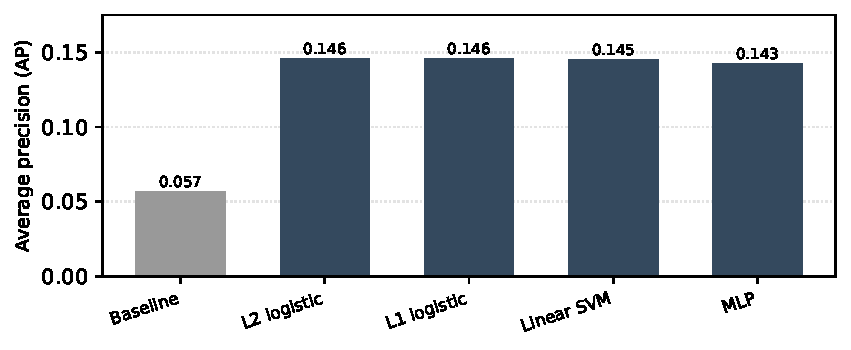
\includegraphics[width=.98\columnwidth]{january_selection_ap.pdf}
\caption{January 2018 selection AP from archived experiments. The baseline equals the observed delayed-delivery prevalence. These are historical model-selection scores, not prospective accuracy.}
\label{fig:ap}
\end{figure}

For the selected L2 model, March 2018 contained 7,003 comparable records (ROC-AUC 0.634753, AP 0.304187). The April--July aggregate contained 25,799 records (ROC-AUC 0.678720, AP 0.075016). The February-calibrated score averaged 21.9829\% in April--July, whereas the observed late fraction was 3.9847\%: an \emph{absolute gap of 17.9982 percentage points}. These periods differ substantially in prevalence, and their repeated inspection rules out claims of pristine external validation. An older frozen classifier's separate validation ROC-AUC (0.558705) is reported in the archive, but uses a different cohort, features, and workflow; its value is \emph{not} a like-for-like benchmark against this challenger.

\subsection{Synthetic Allocation and Stress Cases}
For the fictional July case, the declared baseline landed cost is USD 1,928,061. The exact feasible monthly assignment has modeled cost USD 1,698,024, a difference of USD 230,037 (11.93\% of the modeled baseline), while satisfying the coded monthly constraints. The paired stress experiment reproduces 500 assumed shared shocks for all 80 candidate pairs. These computations verify the specified \emph{fictional} optimization and experiment mechanics only. They do not show cost savings in a real firm, validate daily commitments, establish supplier substitution effects, or prove recovery under real disruptions.

\begin{table}[t]
\caption{Evidence Status of Main Claims}
\centering\footnotesize\setlength{\tabcolsep}{3pt}
\begin{tabular}{p{.34\columnwidth}p{.57\columnwidth}}
\toprule
Claim & Supported interpretation\\
\midrule
Historical classification & Ranking metrics on retrospectively labeled Olist orders\\
Synthetic cost difference & Exact modeled result under a fictional monthly instance\\
Copilot and charts & Implemented local software; response correctness bounded by available evidence\\
Live supplier advantage & \textbf{Not established}; no verified intervention/cost outcomes\\
Future calibrated risk & \textbf{Not established}; requires prospective as-of inputs and independent labels\\
\bottomrule
\end{tabular}
\label{tab:status}
\end{table}

\section{Discussion and Limitations}
The model benchmark demonstrates that a parsimonious linear classifier remains competitive with more complex candidates on the reported January development split, but it cannot establish generalization to future operational environments. The modest ranking performance, varying event prevalence, and severe April--July calibration gap all constrain decision usefulness. In addition, Olist's estimated delivery date is not independently certified as a contractual commitment; seller/item information was not verified as available in immutable snapshots at the original decision time. The existing historical test was repeatedly inspected, so a genuinely future pre-registered cohort is required.

The optimizer is exact only within its specified component-month model; it does not prove real quotes, capacity, daily route availability, multi-item enterprise obligations, or causal effect of supplier switches. Although paired shock inputs reduce some comparison asymmetry inside the synthetic test, the shock formula remains assumed rather than fitted. The application provides a usable local research demonstration, not enterprise authentication, production monitoring, or certified supplier decision execution. Real-world adoption would require independent event-time records, evaluation on new labels, governance and approval, comprehensive operating costs, and controlled intervention evidence.

\section{Reproducibility and Responsible AI Use}
Original historical Olist source CSVs are obtainable from the public dataset \cite{olist2018} subject to its stated license. The project archive contains preserved research notebooks, synthetic inputs, frozen model artifacts, source hash inventories, unit tests, and dated validation JSON reports. The reproducibility guide accompanying this paper identifies exact commands for benchmark regeneration, archived synthetic stress reproduction, package verification, and local launch. A GitHub URL is to be inserted after the author publishes the approved repository; none is asserted here. Code versions and input hashes must be preserved for reported results.

\textit{AI-use declaration:} The author reports developing the primary Jupyter-based research foundation and project direction independently. ChatGPT was used during subsequent implementation refinement, debugging, testing, evidence review, and language editing. All submitted material, analysis claims, and course AI-use compliance remain the author's responsibility. The author will verify the final AI-origin proportion according to the course's declared limit before submission; this manuscript does not assert an independently measured percentage.

\section{Conclusion}
AEGIS demonstrates an auditable educational workflow that brings together historical risk ranking, fictional capacity-constrained optimization, and evidence-grounded managerial communication. A 38-configuration historical benchmark and a reproducible synthetic allocation provide concrete results, while weak calibration, unverified feature timing, and the absence of real supplier outcomes place clear limits on operational claims. The project's contribution is a decision-support architecture that makes these boundaries visible rather than disguising research assumptions as business facts.

\begin{thebibliography}{00}
\bibitem{bertsimas2020} D. Bertsimas and N. Kallus, ``From predictive to prescriptive analytics,'' \emph{Management Science}, vol. 66, no. 3, pp. 1025--1044, 2020, doi: 10.1287/mnsc.2018.3253.
\bibitem{fawcett2006} T. Fawcett, ``An introduction to ROC analysis,'' \emph{Pattern Recognition Letters}, vol. 27, no. 8, pp. 861--874, 2006, doi: 10.1016/j.patrec.2005.10.010.
\bibitem{saito2015} T. Saito and M. Rehmsmeier, ``The precision-recall plot is more informative than the ROC plot when evaluating binary classifiers on imbalanced datasets,'' \emph{PLOS ONE}, vol. 10, no. 3, Art. no. e0118432, 2015, doi: 10.1371/journal.pone.0118432.
\bibitem{sculley2015} D. Sculley \emph{et al.}, ``Hidden technical debt in machine learning systems,'' in \emph{Advances in Neural Information Processing Systems}, vol. 28, pp. 2503--2511, 2015.
\bibitem{olist2018} Olist, ``Brazilian E-Commerce Public Dataset by Olist,'' Kaggle, 2018. [Online]. Available: \url{https://www.kaggle.com/datasets/olistbr/brazilian-ecommerce}. [Accessed: Nov. 8, 2026].
\end{thebibliography}
\end{document}
